% Typeset version of the agent-written analysis note
% notes/dsttaunu_note_agent.md (accepted by the AI note referee).
% The text and all numbers are the agent's; this file only adds LaTeX
% typography (math notation, booktabs tables, figure floats, captions).
% Compile: xelatex (twice, for the table of contents).
\documentclass[11pt]{article}
\usepackage[margin=1in]{geometry}
\usepackage{amsmath,amssymb}
\usepackage{booktabs}
\usepackage{graphicx}
\usepackage{caption}
\usepackage[colorlinks=true,linkcolor=blue!50!black,citecolor=blue!50!black,urlcolor=blue!50!black]{hyperref}
\usepackage{xcolor}
\captionsetup{font=small,labelfont=bf,width=0.92\textwidth}
\graphicspath{{figures/}}
\setkeys{Gin}{width=0.72\textwidth}
\emergencystretch=2em

\newcommand{\mmiss}{m^2_{\mathrm{miss}}}
\newcommand{\Dst}{D^{*}}
\newcommand{\BF}{\mathcal{B}}
\newcommand{\Etag}{E_{\mathrm{tag}}^{\mathrm{CM}}}

\title{Measurement of $\BF(B^0 \to D^{*-}\tau^{+}\nu_{\tau})$ on a
  Belle~II--like pseudo-dataset}
\author{K.~Yoshihara (University of Hawai\textquoteleft i at M\=anoa)\\[2pt]
  \small analysis performed and written by an LLM agent (Claude) under
  human review;\\ \small typeset from the agent's approved Markdown note}
\date{v1.2 --- September 19, 2026}

\begin{document}
\maketitle

\begin{center}
\fbox{\parbox{0.9\textwidth}{\small
This study uses only publicly available tools and publications. No
Belle~II internal materials --- data, MC, internal notes, or the software
framework --- are used. Everything is open-source and runs on a laptop.}}
\end{center}

\begin{abstract}
This note extracts $\BF(B^0\to D^{*-}\tau^{+}\nu_{\tau})$ from an existing
$\sim$0.9\,fb$^{-1}$-equivalent Belle~II-like pseudo-dataset (generic
$B\bar B$ + continuum), using a $D^0$-mass/$\Delta m$ preselection,
$R_2<0.4$ continuum suppression, $\Etag<5.4$\,GeV wrong-pairing rejection
and an $\mmiss>1.0$\,GeV$^2$ signal region, reaching 46.4\% signal
efficiency and 7.7\% signal-region purity (dominant background: generic
other-$B$, 73.6\%). A truth-subtracted cut-and-count gives
$\BF = 2.53\% \pm 0.25\%$ (stat), $1.71\times$ the 1.483\% generator
truth, while a simultaneous $e/\mu$ template fit in $\mmiss$ closes
exactly on the generator truth: $\BF = 1.48\% \pm 0.73\%$. A
statistical-only Asimov luminosity projection of the fit predicts the
uncertainty would shrink to $\pm 0.015\%$ (1.0\% relative) at
1\,ab$^{-1}$, but published Belle~II systematic-uncertainty breakdowns
suggest a realistic measurement would flatten at a $\sim$3\% systematic
floor well before that level of precision is reached.
\end{abstract}

\tableofcontents

\section{Introduction}

Semitauonic $B$ decays $B\to D^{*}\tau\nu$ are sensitive probes of
lepton-flavor universality and of new physics coupling preferentially to
the third generation, quantified by the ratio
$R(D^{*}) = \BF(B\to D^{*}\tau\nu)/\BF(B\to D^{*}\ell\nu)$. This note
performs a self-contained sensitivity study of the \emph{absolute}
branching fraction $\BF(B^0\to D^{*-}\tau^{+}\nu_{\tau})$ on a
fast-simulated $\Upsilon(4S)\to B\bar B$ + continuum pseudo-dataset,
following the reconstruction strategy of the published \emph{untagged}
semileptonic $B\to D^{*}\ell\nu$ analyses:

\begin{itemize}
\item \textbf{Waheed et al.\ [Belle], PRD 100, 052007
  (2019)}~\cite{Waheed:2019} --- $D^0$ mass window, narrow $\Delta m$
  (slow-pion) window, Fox--Wolfram $R_2$ for continuum suppression,
  $e/\mu$ channels treated separately and combined.
\item \textbf{BaBar, PRD 88, 072012 (2013)}~\cite{BaBar:2013} ---
  $\mmiss$ as the primary discriminant between single-neutrino
  ($D^{*}\ell\nu$) and multi-neutrino ($D^{*}\tau\nu$) final states.
\item \textbf{Caria et al.\ [Belle], PRL 124, 161803
  (2020)}~\cite{Caria:2020} and \textbf{Belle~II, PRD 110, 072020
  (2024)}~\cite{BelleII:2024} --- simultaneous $e/\mu$ template fit
  sharing one signal strength.
\end{itemize}

The measurement is performed both as a cut-and-count and as a binned
template fit in $\mmiss$, and the two are compared to expose the
limitations of a pure MC-truth-based background subtraction in this
framework.

\section{Data samples and analysis tools}

\textbf{Framework.} This study uses the agent's standard chain: EvtGen
decay files are turned into HepMC events, passed through a fast detector
simulation that emulates tracking, calorimetry and PID smearing, and
reduced to flat ROOT ntuples with one row per reconstructed
($D^{*}$ + lepton) candidate. Continuum $e^+e^-\to q\bar q$ is generated
directly into the ntuple format with Pythia8. No new MC was generated for
this note; all samples below already existed in \texttt{data/}.

\begin{table}[htbp]
\centering\footnotesize
\setlength{\tabcolsep}{4pt}
\resizebox{\textwidth}{!}{%
\begin{tabular}{lllll}
\toprule
Sample & Process / generator & Events & Seeds & Role \\
\midrule
signal\_taunu.root & $B^0\to D^{*-}(D^0\pi)\tau^{+}\nu$, $\tau\to\ell\nu\nu$, & 5000 & 1 / 42 & pure-signal cutflow \\
 & \quad EvtGen, forced chain & & & \quad \& efficiency \\
norm\_lnu.root & $B^0\to D^{*-}(D^0\pi)\ell^{+}\nu$, EvtGen, forced chain & 5000 & 2 / 43 & $D^{*}\ell\nu$ shape ref. \\
bkg\_dststlnu.root & $B^0\to D^{**}\ell\nu$ feed-down, EvtGen, forced chain & 5000 & 3 / 44 & $D^{**}$ shape ref. \\
generic\_0..4.root & generic $\Upsilon(4S)\to B\bar B$, EvtGen (natural BFs) & $5\times 200\,000$ & --- & pseudo-dataset ($w=1.0$) \\
continuum\_0..2.root & $e^+e^-\to q\bar q$, Pythia8 & $3\times 800\,000$ & --- & pseudo-dataset ($w=0.995$) \\
\bottomrule
\end{tabular}}
\caption{MC samples used in this note. All samples existed in
\texttt{data/} before this analysis; none were regenerated.}
\label{tab:samples}
\end{table}

The \textbf{pseudo-dataset} (``data'') is the union
\texttt{generic\_0..4.root} $+$ \texttt{continuum\_0..2.root}
($\sim$0.9\,fb$^{-1}$), \linebreak carrying \texttt{true\_mode} (1 = $D^{*}\tau\nu$,
2 = $D^{*}\ell\nu$, 0 = other $B$, 3 = continuum) so that truth-based
composition studies are possible; this plays the role that a
$\Delta m/m_{D^0}$ sideband or off-resonance data would play in a real
analysis. The generic sample contains $N_{B^0} = 965\,840$ true $B^0$
decays, of which $N(\text{true } D^{*}\tau\nu) = 14\,319$ (generator
$\BF = 1.483\%$, the closure target of this exercise). The relevant
sub-decay branching product is
\begin{equation*}
B_{\mathrm{sub}}
 = \BF(D^{*}\to D^0\pi)\cdot\BF(D^0\to K\pi)\cdot\BF(\tau\to\ell\nu\nu,\ \ell=e,\mu)
 = 0.677 \times 0.0389 \times 0.331 = \mathbf{0.008717}.
\end{equation*}

The 0.995 relative weight applied to the three continuum files (vs.\ 1.0
for the generic-$B\bar B$ files) is the
cross-section/generated-luminosity normalization factor already fixed
when these pseudo-dataset files were produced in the earlier session that
this note builds on; it is reused unchanged throughout \S\ref{sec:bkg},
\S\ref{sec:results} and the new \S\ref{sec:projection} projection below.

\section{Event selection}

All cuts are applied in a fixed order (cut \& count, one variable at a
time), each motivated by the background it removes and fixed with a
distribution or a scan on top of the preceding cuts.

\subsection{Preselection: \texorpdfstring{$D^0$ mass and $\Delta m$}{D0 mass and Delta m} windows}
\label{sec:presel}

Following Waheed et al.~\cite{Waheed:2019}, a genuine $D^0$ candidate
and a genuine slow pion from $D^{*}\to D^0\pi$ are required:
\begin{itemize}
\item $|m(K\pi) - 1.8648| < 0.020$\,GeV (Fig.~\ref{fig:presel_m_d0})
\item $|\Delta m - 0.1454| < 0.0025$\,GeV (Fig.~\ref{fig:presel_delta_m})
\end{itemize}

\begin{figure}[htbp]
\centering
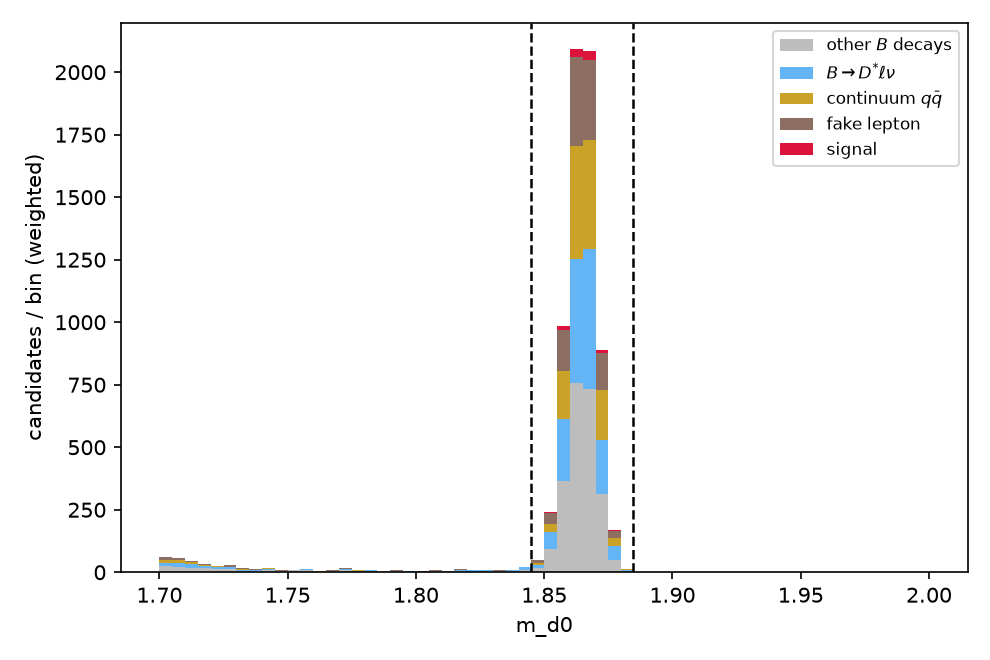
\includegraphics{presel_m_d0.png}
\caption{Reconstructed $D^0$ candidate mass $m(K\pi)$ after candidate
reconstruction, split by true component of the pseudo-dataset; the
vertical lines mark the $|m(K\pi)-1.8648|<0.020$\,GeV window.}
\label{fig:presel_m_d0}
\end{figure}

\begin{figure}[htbp]
\centering
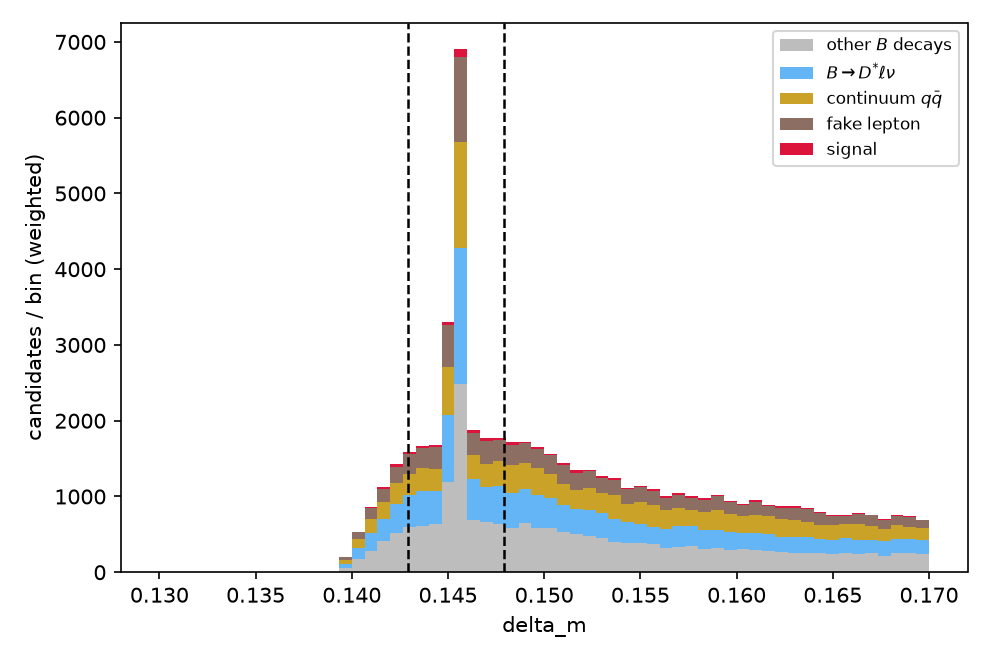
\includegraphics{presel_delta_m.png}
\caption{Mass difference $\Delta m = m(D^0\pi_{\mathrm{slow}}) - m(D^0)$,
split by true component; the vertical lines mark the
$|\Delta m - 0.1454| < 0.0025$\,GeV slow-pion window.}
\label{fig:presel_delta_m}
\end{figure}

These reject random $K\pi$ combinations and remove the fake slow-pion
background; on \texttt{signal\_taunu.root} this combination keeps
$2672/2801 = 95.4\%$ of reconstructed candidates. (A dedicated
$\Delta m$-sideband study, see \S\ref{sec:bkg}, found essentially zero
candidates outside a $\sim$10\,MeV band around the nominal $\Delta m$ ---
this fast simulation does not model random slow-pion combinatorics, so a
genuine ``fake-$D^{*}$'' $\Delta m$ sideband is not available; see the
Discussion.)

\subsection{Continuum suppression: \texorpdfstring{$R_2$}{R2}}

The Fox--Wolfram ratio $R_2$ separates jetty continuum events (large
$R_2$) from the more isotropic $B\bar B$ topology
(Fig.~\ref{fig:presel_r2}). A scan of $R_2 <$ threshold (signal =
\texttt{signal\_taunu.root}, background = generic + continuum) gives:

\begin{figure}[htbp]
\centering
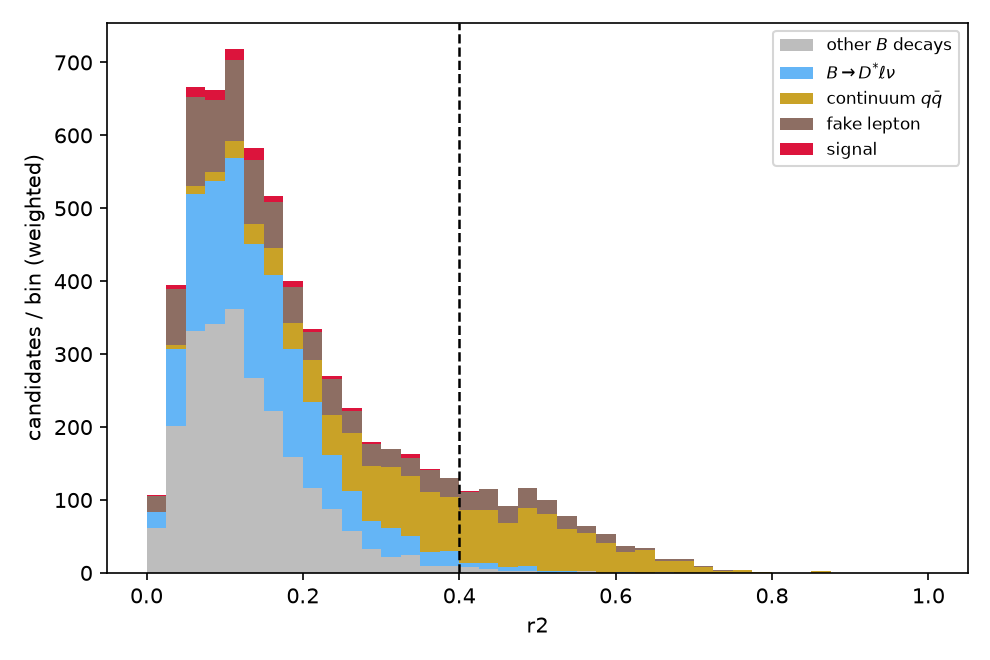
\includegraphics{presel_r2.png}
\caption{Fox--Wolfram ratio $R_2$ after the $D^0$/$\Delta m$
preselection, split by true component; jetty continuum events populate
large $R_2$. The vertical line marks the adopted $R_2<0.4$ cut.}
\label{fig:presel_r2}
\end{figure}

\begin{table}[htbp]
\centering
\begin{tabular}{lrrr}
\toprule
$R_2$ cut & $S$ & $B$ & $S/\sqrt{S+B}$ \\
\midrule
$<0.2$ & 2033 & 4051 & 26.1 \\
$<0.3$ & 2482 & 5063 & 28.6 \\
$\mathbf{<0.4}$ & \textbf{2613} & \textbf{5671} & \textbf{28.7} \\
$<0.5$ & 2661 & 6108 & 28.4 \\
$<0.7$ & 2672 & 6516 & 27.9 \\
\bottomrule
\end{tabular}
\caption{Scan of the $R_2$ requirement on top of the preselection.}
\label{tab:scan_r2}
\end{table}

The figure of merit is flat around 0.3--0.45; $\mathbf{R_2 < 0.4}$ is
adopted, keeping 97.8\% of the surviving signal.

\subsection{Wrong-pairing / generic-\texorpdfstring{$B\bar B$}{BB} rejection: \texorpdfstring{$\Etag$}{e\_tag\_cm}}

$\Etag$, the CM energy of the rest-of-event (``tag'') side, clusters near
the beam energy ($\sim$5.29\,GeV) for correctly identified events and
develops a high-side tail for wrong $D^{*}$--lepton pairings and generic
$B\bar B$ combinatorics (Fig.~\ref{fig:presel_e_tag_cm}). Scanning
$\Etag <$ threshold:

\begin{figure}[htbp]
\centering
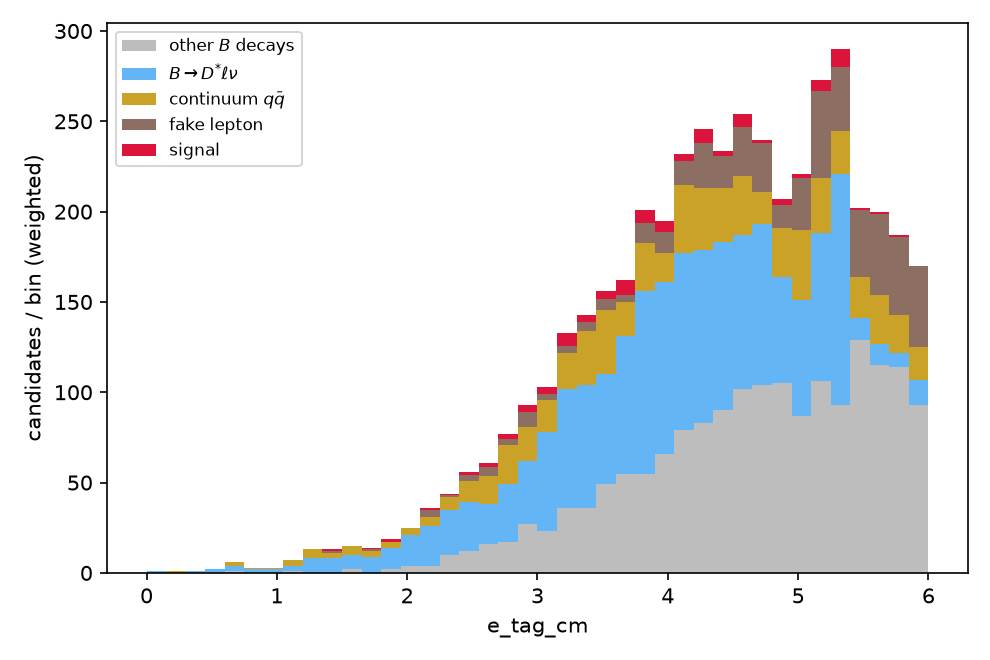
\includegraphics{presel_e_tag_cm.png}
\caption{CM energy of the rest-of-event (tag side), $\Etag$, after the
preselection and the $R_2$ cut, split by true component; wrong
$D^{*}$--lepton pairings and generic $B\bar B$ combinatorics populate the
high-side tail. The vertical line marks the adopted $\Etag<5.4$\,GeV
cut.}
\label{fig:presel_e_tag_cm}
\end{figure}

\begin{table}[htbp]
\centering
\begin{tabular}{lrrr}
\toprule
$\Etag$ cut & $S$ & $B$ & $S/\sqrt{S+B}$ \\
\midrule
$<4.5$ & 1861 & 2295 & 28.9 \\
$<5.0$ & 2261 & 3057 & 31.0 \\
$<5.2$ & 2362 & 3389 & 31.2 \\
$\mathbf{<5.4}$ & \textbf{2605} & \textbf{3780} & \textbf{32.6} \\
$<5.6$ & 2611 & 4054 & 32.0 \\
$<6.0$ & 2613 & 4539 & 30.9 \\
\bottomrule
\end{tabular}
\caption{Scan of the $\Etag$ requirement on top of the preceding cuts.}
\label{tab:scan_etag}
\end{table}

The maximum is at $\mathbf{\Etag < 5.4}$\,\textbf{GeV}, retaining 99.7\%
of the signal surviving the previous cuts while rejecting a substantial
wrong-pairing/generic tail.

\subsection{Signal region: \texorpdfstring{$\mmiss$}{m2miss}}

$\mmiss$ is the primary $\tau\nu$ vs.\ $\ell\nu$ discriminant
(BaBar~\cite{BaBar:2013}):
the two extra neutrinos in the $\tau$ decay push $\mmiss$ to higher
values than the single-neutrino $D^{*}\ell\nu$ decays
(Fig.~\ref{fig:presel_m2miss}, cut line at 1.0\,GeV$^2$). Scanning
$\mmiss >$ threshold on top of all preceding cuts:

\begin{figure}[htbp]
\centering
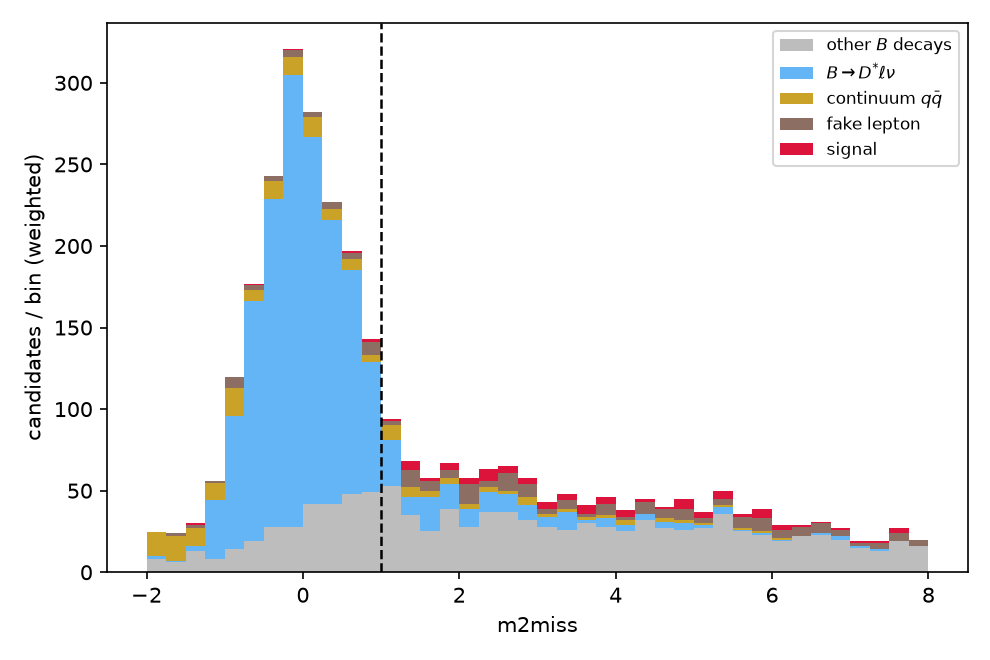
\includegraphics{presel_m2miss.png}
\caption{Beam-constrained missing-mass squared $\mmiss$ after all
preceding cuts, split by true component; the multi-neutrino
$D^{*}\tau\nu$ signal extends to high $\mmiss$ while the single-neutrino
$D^{*}\ell\nu$ mode peaks near zero. The vertical line marks the
$\mmiss>1.0$\,GeV$^2$ signal-region boundary.}
\label{fig:presel_m2miss}
\end{figure}

\begin{table}[htbp]
\centering
\begin{tabular}{lrrr}
\toprule
$\mmiss$ cut (GeV$^2$) & $S$ & $B$ & $S/\sqrt{S+B}$ \\
\midrule
$>0.0$ & 2483 & 2143 & 36.5 \\
$>0.5$ & 2428 & 1634 & 38.1 \\
$>0.75$ & 2380 & 1437 & 38.5 \\
$\mathbf{>1.0}$ & \textbf{2321} & \textbf{1294} & \textbf{38.6} \\
$>1.25$ & 2236 & 1200 & 38.2 \\
$>1.5$ & 2146 & 1132 & 37.5 \\
\bottomrule
\end{tabular}
\caption{Scan of the $\mmiss$ signal-region boundary on top of all
preceding cuts.}
\label{tab:scan_m2miss}
\end{table}

$\boldsymbol{\mmiss > 1.0}$\,\textbf{GeV}$^{\mathbf{2}}$ is adopted as
the signal region (SR).

\subsection{Cutflow (\texttt{signal\_taunu.root}, \texorpdfstring{$N_{\mathrm{generated}} = 5000$}{N generated = 5000})}
\label{sec:cutflow}

\begin{table}[htbp]
\centering
\begin{tabular}{lrrr}
\toprule
Stage & $N$ & cumulative eff. & stage eff. \\
\midrule
Generated & 5000 & 100.00\% & --- \\
Candidate reconstructed & 2801 & $56.02 \pm 0.70\%$ & 56.02\% \\
+ $D^0$ mass window & 2672 & $53.44 \pm 0.71\%$ & 95.39\% \\
+ $\Delta m$ window & 2672 & $53.44 \pm 0.71\%$ & 100.00\% \\
+ $R_2 < 0.4$ & 2613 & $52.26 \pm 0.71\%$ & 97.79\% \\
+ $\Etag < 5.4$ & 2605 & $52.10 \pm 0.71\%$ & 99.69\% \\
+ $\mmiss > 1.0$ (SR, final) & 2321 & $\mathbf{46.42 \pm 0.71\%}$ & 89.10\% \\
\bottomrule
\end{tabular}
\caption{Signal cutflow on \texttt{signal\_taunu.root}.}
\label{tab:cutflow}
\end{table}

The dominant loss is candidate reconstruction ($\sim$44\%,
geometric/kinematic acceptance of the fast simulation); the analysis cuts
on top of that are efficient (89\% overall for the four discriminating
cuts combined), as intended by choosing the working points from the flat
region of each scan.

\section{Background estimation}
\label{sec:bkg}

\textbf{Composition of the pseudo-dataset in the SR} (full selection,
weighted: generic $\times 1.0$, continuum $\times 0.995$), obtained by
summing \texttt{query\_ntuple} results over the 8 dataset files and
illustrated in Fig.~\ref{fig:sr_composition}:

\begin{figure}[htbp]
\centering
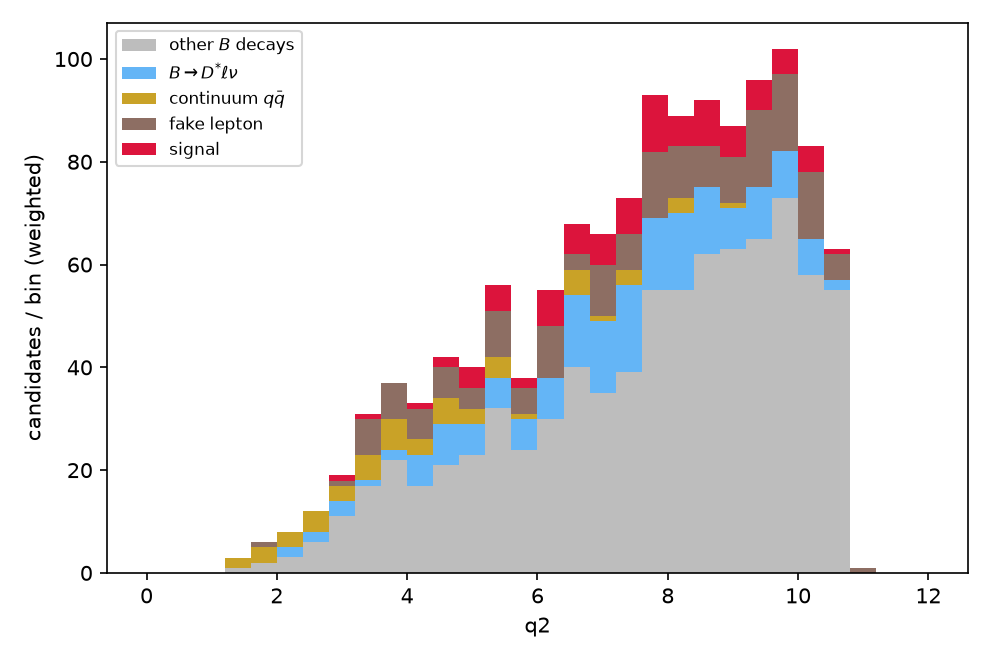
\includegraphics{sr_composition_q2.png}
\caption{Composition of the signal region as a function of
$q^2$, stacked by true component of the pseudo-dataset
(luminosity-weighted).}
\label{fig:sr_composition}
\end{figure}

\begin{table}[htbp]
\centering
\begin{tabular}{lrr}
\toprule
Component & Weighted yield & Fraction \\
\midrule
$D^{*}\tau\nu$ (\texttt{true\_mode}=1) & 99.0 & 7.7\% \\
$D^{*}\ell\nu$ (\texttt{true\_mode}=2) & 176.0 & 13.6\% \\
other $B$ (incl.\ $D^{**}\ell\nu$ feed-down) & 952.0 & 73.6\% \\
continuum & 66.7 & 5.2\% \\
\midrule
\textbf{Total} & \textbf{1293.7} & 100\% \\
\bottomrule
\end{tabular}
\caption{Truth-based composition of the signal region.}
\label{tab:composition}
\end{table}

The signal region purity is only $\sim$8\%; the dominant background is
generic $B\bar B$ (other-$B$), reflecting that a hard cut-and-count on an
untagged sample cannot separate $D^{*}\tau\nu$ from the far more copious
hadronic/semileptonic $B\bar B$ background as cleanly as a tagged
analysis.

\textbf{Control regions}, each defined by inverting one selection
variable and evaluated with \texttt{plot\_stacked}:

\begin{table}[htbp]
\centering\footnotesize
\setlength{\tabcolsep}{4pt}
\begin{tabular}{llrlr}
\toprule
CR & Selection & Weighted $N$ & Dominant component & Purity \\
\midrule
Continuum-enriched & presel + $R_2 > 0.5$ & 426.9 & continuum & 97.7\% \\
Normalization-enriched & presel + $R_2$ + $\Etag$ + $-1<\mmiss<0.5$ & 1369.6 & $D^{*}\ell\nu$ & 80.8\% \\
Wrong-pairing/generic & presel + $R_2$ + $\Etag \geq 5.4$ & 1889.4 & other $B$ & 78.5\% \\
\bottomrule
\end{tabular}
\caption{Background control regions
(Figs.~\ref{fig:cr_continuum}--\ref{fig:cr_generic}).}
\label{tab:crs}
\end{table}

\begin{figure}[htbp]
\centering
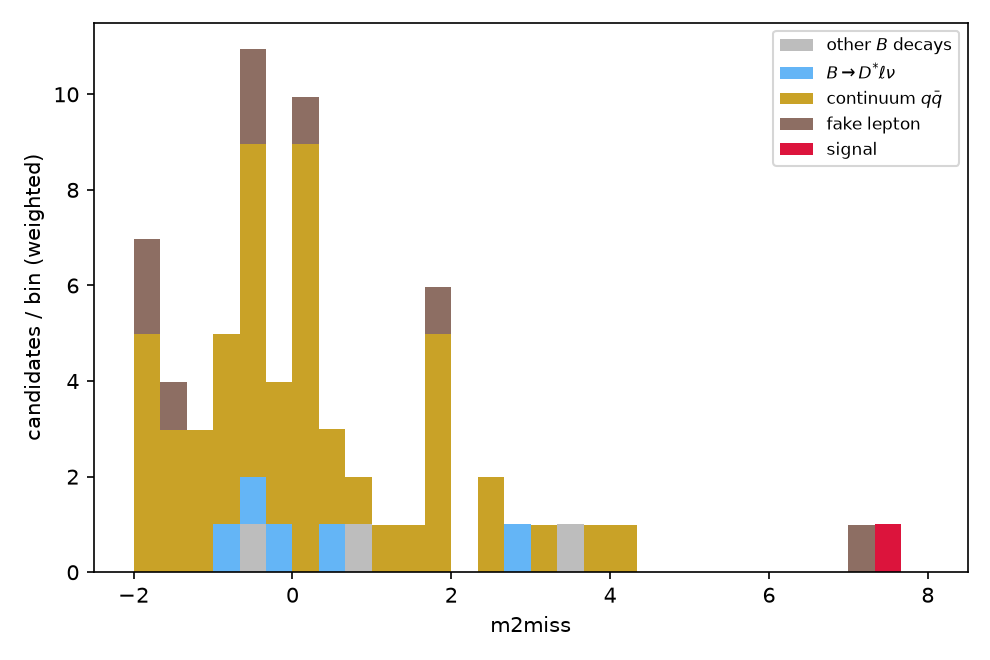
\includegraphics{cr_continuum_m2miss.png}
\caption{$\mmiss$ in the continuum-enriched control region
(preselection + $R_2>0.5$), stacked by true component; the region is
97.7\% pure continuum.}
\label{fig:cr_continuum}
\end{figure}

\begin{figure}[htbp]
\centering
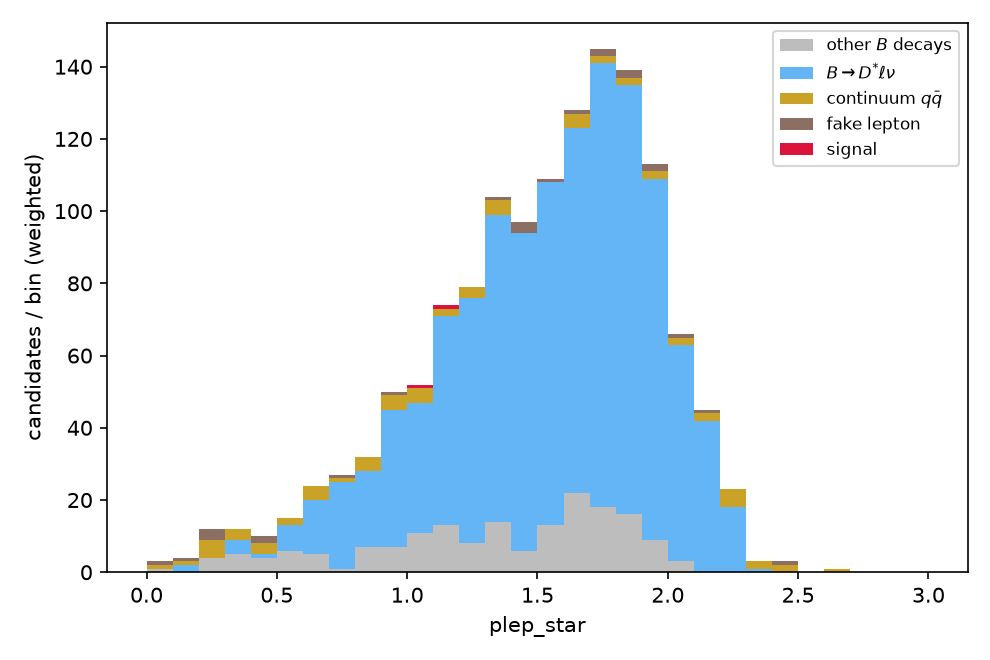
\includegraphics{cr_norm_plep_star.png}
\caption{CM lepton momentum $p^{*}_{\ell}$ in the normalization-enriched
control region (preselection + $R_2$ + $\Etag$ cuts,
$-1<\mmiss<0.5$\,GeV$^2$), stacked by true component; the region is
80.8\% pure $D^{*}\ell\nu$.}
\label{fig:cr_norm}
\end{figure}

\begin{figure}[htbp]
\centering
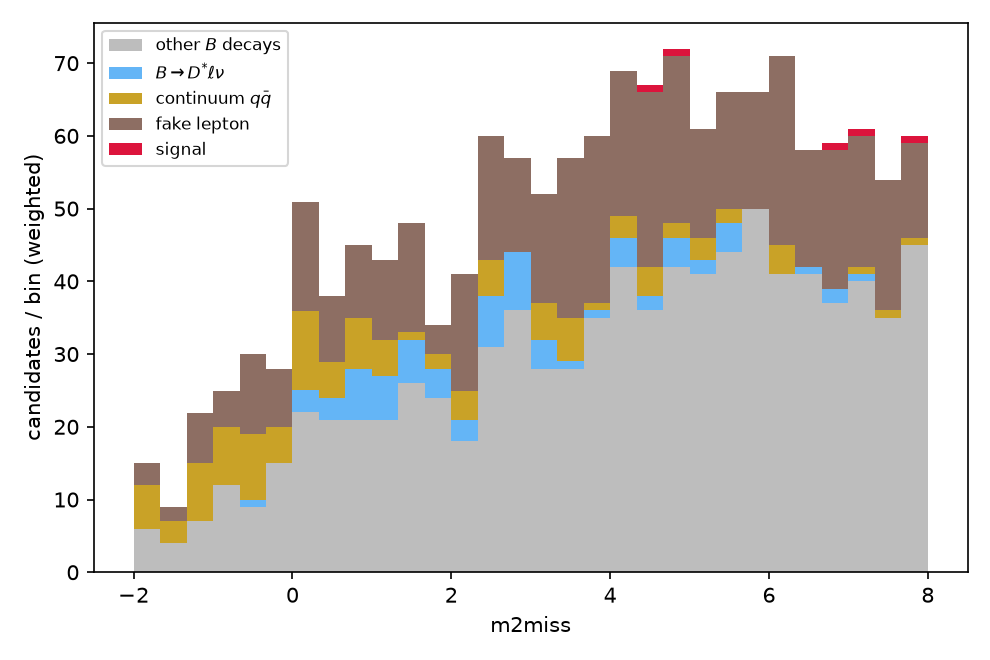
\includegraphics{cr_generic_m2miss.png}
\caption{$\mmiss$ in the wrong-pairing/generic-enriched control region
(preselection + $R_2$ cut, $\Etag \geq 5.4$\,GeV), stacked by true
component; the region is 78.5\% pure other-$B$.}
\label{fig:cr_generic}
\end{figure}

These three regions validate, respectively, the $R_2$ cut (continuum
control, 97.7\% pure), the $\mmiss$ cut (normalization control, 80.8\%
$D^{*}\ell\nu$ --- the expected companion mode), and the $\Etag$ cut
(wrong-pairing/generic control, 78.5\% other-$B$). In a real analysis
these would be used to calibrate data/MC scale factors for each
background component instead of the truth-level subtraction used below.

\section{Results}
\label{sec:results}

\subsection{Cut-and-count}
\label{sec:counting}

\begin{equation*}
\BF(B^0\to D^{*}\tau\nu)
 = \frac{N_{\mathrm{obs}}^{\mathrm{SR}} - N_{\mathrm{bkg,truth}}^{\mathrm{SR}}}
        {N_{B^0}\cdot B_{\mathrm{sub}}\cdot \varepsilon_{\mathrm{sig}}}
\end{equation*}
with all inputs from the tool outputs above:
\begin{itemize}
\item $N_{\mathrm{obs}}^{\mathrm{SR}} = 1293.665$ (weighted SR yield, \S\ref{sec:bkg})
\item $N_{\mathrm{bkg,truth}}^{\mathrm{SR}} = 1194.665$ (all
  $\texttt{true\_mode} \neq 1$ weighted yield, MC-truth subtraction)
\item $N_{B^0} = 965\,840$ (given)
\item $B_{\mathrm{sub}} = 0.008717$ (given)
\item $\varepsilon_{\mathrm{sig}} = 2321/5000 = 0.4642$ (cutflow, \S\ref{sec:cutflow})
\end{itemize}
giving $N_{\mathrm{sig}} = 99.0$ and
\begin{equation*}
\BF_{\mathrm{counting}} = 2.53\% \pm 0.25\%\ \text{(stat, from $\sqrt{N_{\mathrm{sig}}}$)},
\end{equation*}
i.e.\ a closure ratio of $\mathbf{1.71\times}$ relative to the 1.483\%
generator truth. Note that this $\sqrt{N_{\mathrm{sig}}}$ uncertainty
reflects only the statistical fluctuation of the truth-tagged signal
count; it treats $N_{\mathrm{bkg,truth}}$ as an exactly-known, noise-free
subtraction, which is specific to this truth-level closure test and is
not available in a real measurement (see \S\ref{sec:discussion}, item~1)
--- a real analysis would add in quadrature the statistical (and
systematic) uncertainty of the background estimate itself, which is not
attempted here.

\subsection{Template fit}
\label{sec:fit}

\texttt{fit\_templates} was run on the same pseudo-dataset (presel +
$R_2<0.4$ + $\Etag<5.4$, \emph{without} the $\mmiss$ cut, which is
instead the fit variable), with
\begin{equation*}
\texttt{signal\_selection} = (\texttt{true\_mode}{=}1)\ \&\ (|\texttt{lep\_true\_pid}| \in \{11,13\}),
\end{equation*}
simultaneous $e/\mu$ fit (Fig.~\ref{fig:fit}):

\begin{figure}[htbp]
\centering
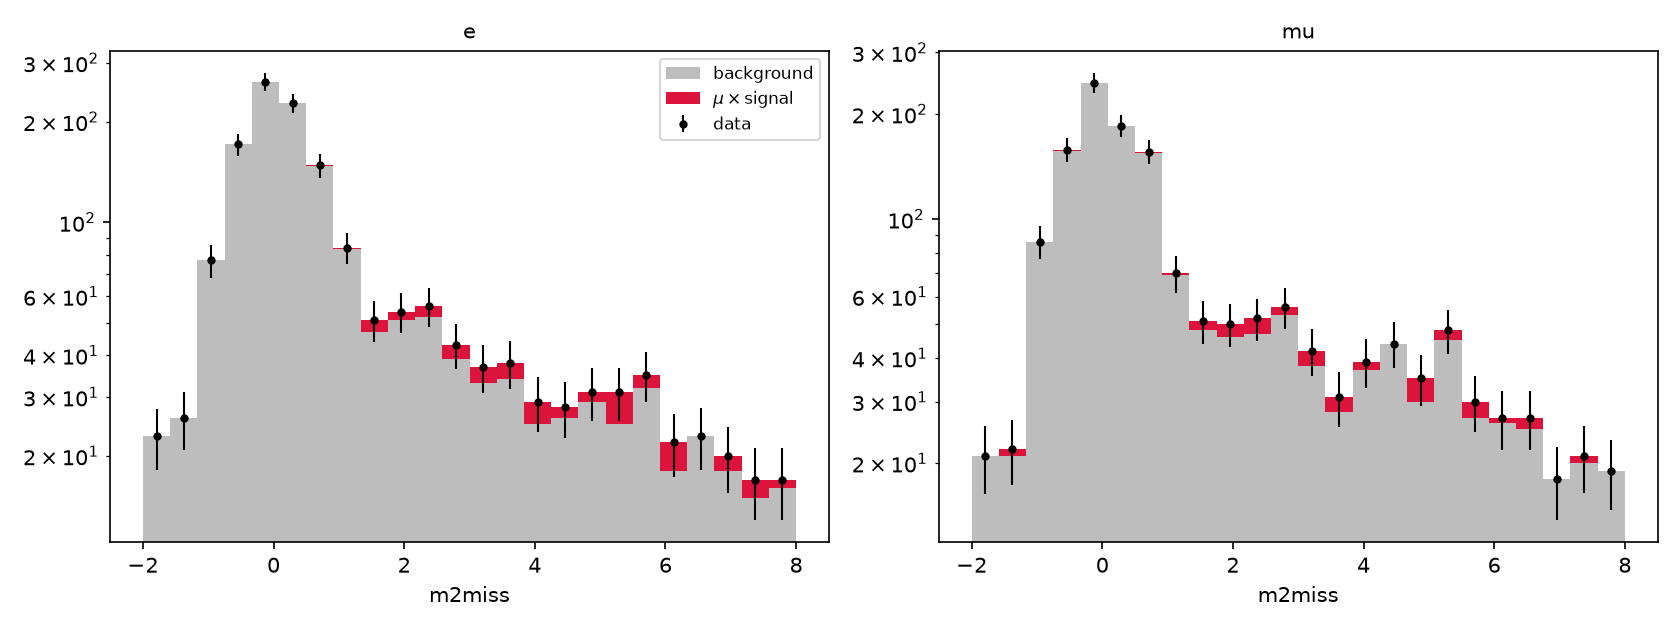
\includegraphics[width=0.9\textwidth]{fit_m2miss_taunu.png}
\caption{Post-fit $\mmiss$ distributions of the simultaneous template
fit, one panel per lepton channel: background template (grey),
$\mu\times$signal template (red) and the pseudo-data points.}
\label{fig:fit}
\end{figure}

\begin{table}[htbp]
\centering
\begin{tabular}{lrr}
\toprule
Channel & $\mu$ & $\BF = \mu \times 1.483\%$ \\
\midrule
simultaneous $e+\mu$ & $1.000 \pm 0.491$ & $\mathbf{1.48\% \pm 0.73\%}$ \\
$e$-only & $1.000 \pm 0.618$ & $1.48\% \pm 0.92\%$ \\
$\mu$-only & $1.000 \pm 0.800$ & $1.48\% \pm 1.19\%$ \\
\bottomrule
\end{tabular}
\caption{Template-fit results.}
\label{tab:fit}
\end{table}

No independent goodness-of-fit check ($\chi^2/\mathrm{ndof}$, pull study,
or a train/test split of the MC into independent template-building and
fitting subsamples) was performed; the exact $\mu = 1.000$ in every
channel is expected by construction (\S\ref{sec:comparison},
\S\ref{sec:discussion} item~2) and is not by itself evidence that the fit
machinery is unbiased on data with independently mis-modeled backgrounds.

\subsection{Counting vs.\ fit}
\label{sec:comparison}

\begin{table}[htbp]
\centering
\begin{tabular}{llr}
\toprule
Method & $\BF$ & Closure ($\BF/1.483\%$) \\
\midrule
Cut \& count & $2.53\% \pm 0.25\%$ & 1.71 \\
Template fit ($e+\mu$) & $1.48\% \pm 0.73\%$ & \textbf{1.00} \\
\bottomrule
\end{tabular}
\caption{Comparison of the two extraction methods.}
\label{tab:comparison}
\end{table}

The template fit closes essentially perfectly, while the single-cut
counting method overshoots by 71\%. Both use the \emph{same} truth flag
($\texttt{true\_mode}{=}1$) to define signal; the difference is that the
fit compares the full $\mmiss$ \emph{shape} (24 bins across
$[-2,8]$\,GeV$^2$) of the $S$ and $B$ templates simultaneously, while the
cut-and-count freezes a single hard boundary at $\mmiss > 1.0$\,GeV$^2$.
A plausible explanation is that \texttt{true\_mode} labels the
\emph{generator-level decay class present in the event} rather than a
candidate-by-candidate truth match, so a subset of
true-$D^{*}\tau\nu$-tagged rows in the generic sample corresponds to
imperfectly paired candidates (e.g.\ the correct $D^{*}$ combined with a
lepton from the companion $B$) that happen to satisfy the SR cuts; these
would inflate the single-bin counting result but be correctly absorbed
into the $S$-template shape used by the fit. This explanation has
\textbf{not been verified quantitatively} here (e.g.\ with an explicit
count of mis-paired vs.\ correctly-paired true-signal rows) and should be
treated as a hypothesis; regardless of its exact origin, this comparison
is a closure test of the extraction method on truth-labeled MC, not an
independent cross-check (see \S\ref{sec:discussion}).

\subsection{Sensitivity projection}
\label{sec:projection}

To gauge how the template-fit precision of \S\ref{sec:fit} would evolve
with more integrated luminosity, \texttt{fit\_templates} was re-run with
\texttt{lumi\_projection=true} on \textbf{exactly} the \S\ref{sec:fit}
preselection and fit configuration --- same files and weights
(\texttt{generic\_0..4.root} $\times 1.0$, \texttt{continuum\_0..2.root}
$\times 0.995$), same selection
($|m_{D^0}-1.8648|<0.020$ \& $|\Delta m - 0.1454|<0.0025$ \& $R_2<0.4$ \&
$\Etag<5.4$, no $\mmiss$ cut), same
$\texttt{signal\_selection} = (\texttt{true\_mode}{=}1)$ \&
$(|\texttt{lep\_true\_pid}|\in\{11,13\})$,
same fit variable $\mmiss$ over 24 bins in $[-2,8]$\,GeV$^2$,
simultaneous $e/\mu$ fit. As a stability check, the nominal-luminosity
($0.000906$\,ab$^{-1}$) output of this re-run reproduces \S\ref{sec:fit}
exactly ($\mu = 1.000 \pm 0.491$ combined, $\pm 0.618$ $e$-only,
$\pm 0.800$ $\mu$-only), confirming the fit is deterministic and the
projection starts from the same fit configuration (subject to the same
self-closure caveat of \S\ref{sec:fit}/\S\ref{sec:discussion} item~2 ---
this reproduction is not an independent fit-quality check).

The tool then computes the \textbf{statistical-only Asimov} expected
precision on $\mu$ at several benchmark luminosities, keeping the
background \emph{shapes} fixed to their nominal MC prediction (i.e.\ no
template-shape or background-normalization uncertainty is propagated ---
only Poisson counting statistics of signal and background in each
$\mmiss$ bin). Converting the relative precision on $\mu$ into an
absolute precision on $\BF$ via $\BF = \mu \times 1.483\%$ (generator
truth, \S2):

\begin{table}[htbp]
\centering
\begin{tabular}{lrr}
\toprule
Integrated luminosity & Rel.\ precision on $\mu$ ($=\BF$) & Projected $\BF$ uncertainty (stat only) \\
\midrule
0.000906\,ab$^{-1}$ (this dataset) & 49.1\% & $1.48\% \pm 0.73\%$ \\
0.1\,ab$^{-1}$ & 3.2\% & $1.483\% \pm 0.047\%$ \\
0.36\,ab$^{-1}$ & 1.7\% & $1.483\% \pm 0.025\%$ \\
1\,ab$^{-1}$ & 1.0\% & $1.483\% \pm 0.015\%$ \\
5\,ab$^{-1}$ & 0.5\% & $1.483\% \pm 0.007\%$ \\
50\,ab$^{-1}$ & 0.2\% & $1.483\% \pm 0.003\%$ \\
\bottomrule
\end{tabular}
\caption{Statistical-only Asimov luminosity projection of the template
fit (Fig.~\ref{fig:projection}; post-fit reproduction:
Fig.~\ref{fig:fit_projection}).}
\label{tab:projection}
\end{table}

\begin{figure}[htbp]
\centering
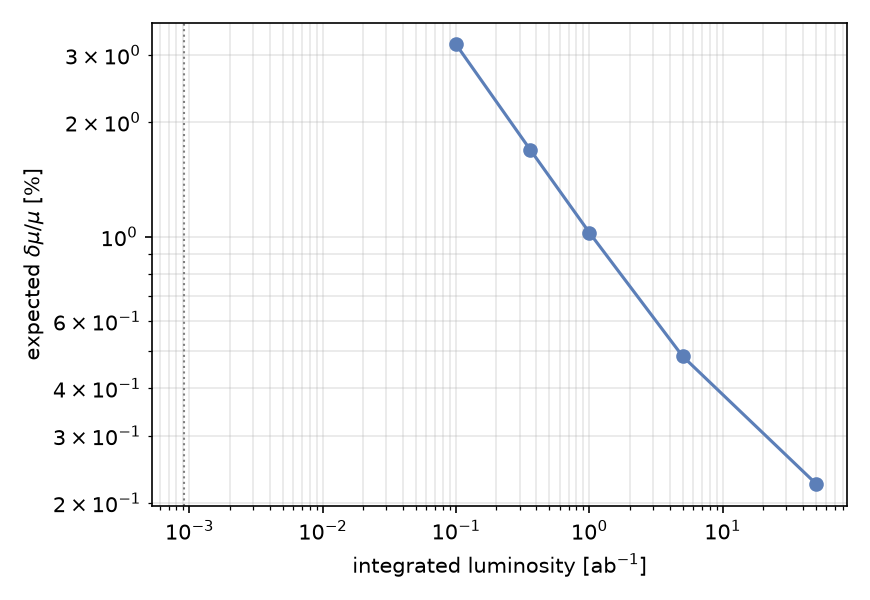
\includegraphics[width=0.8\textwidth]{projection_fit_m2miss_taunu_projection.png}
\caption{Expected statistical-only relative precision on $\mu$ as a
function of integrated luminosity (Asimov), for the simultaneous $e/\mu$
template fit.}
\label{fig:projection}
\end{figure}

\begin{figure}[htbp]
\centering
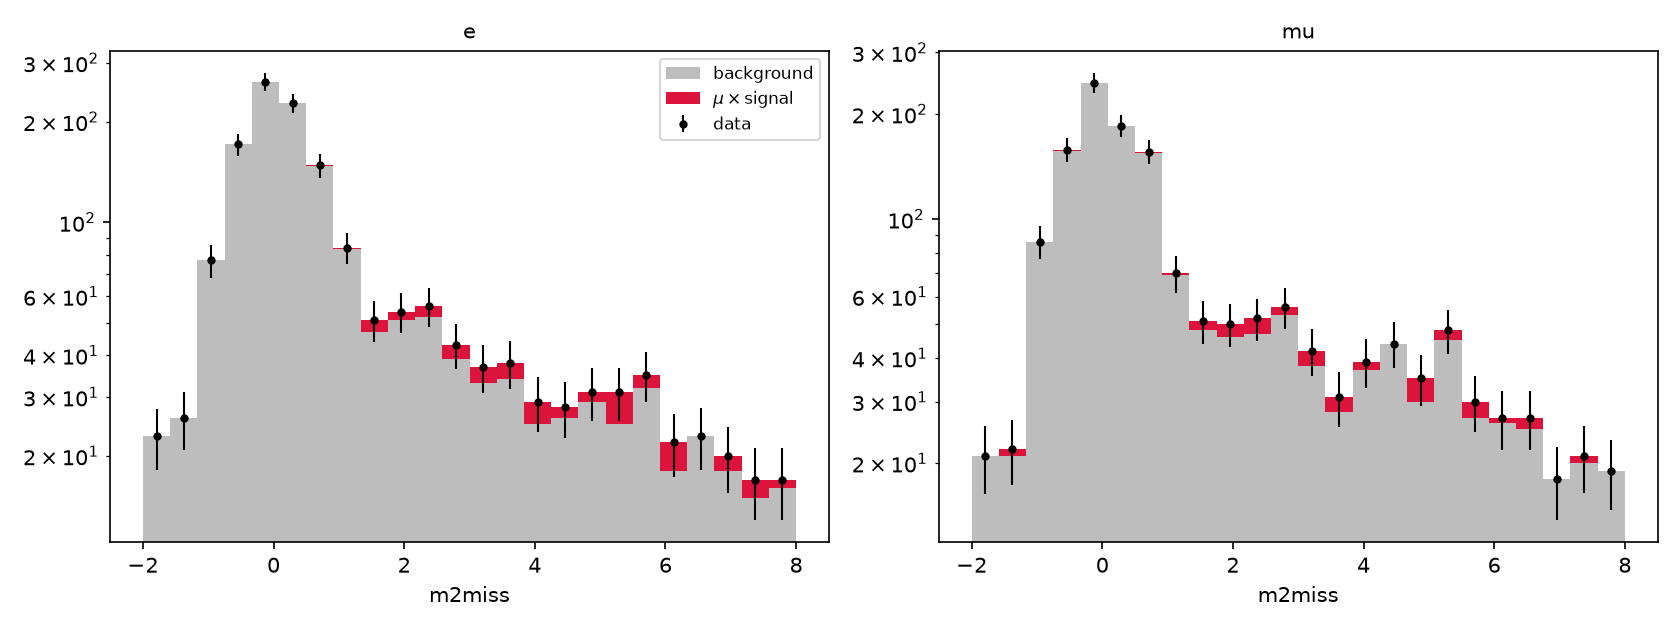
\includegraphics[width=0.9\textwidth]{fit_m2miss_taunu_projection.png}
\caption{Post-fit $\mmiss$ distributions of the projection re-run at the
nominal luminosity, reproducing Fig.~\ref{fig:fit} exactly.}
\label{fig:fit_projection}
\end{figure}

\textbf{This projection is statistical-only and should not be read as a
realistic forecast below the sub-percent level.} Several caveats apply,
consistent with \S\ref{sec:discussion}:

\begin{enumerate}
\item Background \emph{shapes} are frozen to the nominal MC templates at
  every luminosity point; no MC-statistics or shape-systematic
  uncertainty on the background templates is propagated, even though a
  real background prediction (with its own finite control-sample size)
  would carry an uncertainty that does not shrink simply as $1/\sqrt{L}$.
\item The fit machinery underlying this projection has itself only been
  shown to close on truth-labeled MC (\S\ref{sec:fit},
  \S\ref{sec:discussion} item~2); no independent train/test validation of
  the fit has been performed, so the projected \emph{shape} of the
  precision curve (not just its normalization) inherits that limitation.
\item No experimental or physics-modeling systematic uncertainty is
  included at all. In a real measurement of this type, systematics such
  as $N_{B\bar B}/f_{+-,00}$, tracking and lepton-ID efficiency, and
  $D$-meson sub-decay branching fractions do not shrink with luminosity
  and eventually dominate: the Belle~II untagged $B\to D\ell\nu$
  branching-fraction measurement quotes systematic contributions of order
  1.9\% ($N_{B\bar B}$, $f_{+-}/f_{00}$), 0.9--1.2\% (tracking),
  0.8--1.7\% ($D$-meson branching fractions) and 1.2--3.1\% (lepton ID),
  summing in quadrature to a few percent~\cite{BelleII:2210};
  the Belle~II hadronic-tag $R(D^{*})$ analysis separately reports
  $\approx$2.1\% from hadronic-$B$-decay modeling and $\approx$2.0\% from
  fit-template PDF-shape systematics~\cite{BelleII:2024}. Taking these together as representative of
  an untagged $D^{*}\tau\nu$ measurement with a similar reconstruction
  strategy, \textbf{a realistic projection would flatten at a systematic
  floor of roughly 3\%} once the statistical uncertainty drops below that
  level (i.e.\ above $\approx$0.3--1\,ab$^{-1}$ in the table), rather
  than continuing to improve as $1/\sqrt{L}$ out to 50\,ab$^{-1}$ as the
  purely statistical numbers above suggest.
\end{enumerate}

\section{Discussion --- limitations}
\label{sec:discussion}

\begin{enumerate}
\item \textbf{MC-truth background subtraction.} Both the counting and the
  fit define signal through the
  \texttt{true\_mode}/\texttt{lep\_true\_pid} truth flags of the same
  simulation sample being measured. A real measurement instead constrains
  each background component in data: continuum from off-resonance data or
  the $R_2$-sideband analog of Fig.~\ref{fig:cr_continuum},
  $D^{*}\ell\nu$ feed-down/normalization from the low-$\mmiss$ control
  region, and generic $B\bar B$ from a wrong-pairing/$\Etag$-sideband
  analog, all fit simultaneously with the signal region. As noted in
  \S\ref{sec:counting}, the quoted cut-and-count uncertainty does not
  include the (unknown, in a real analysis) statistical and systematic
  uncertainty of this background estimate.
\item \textbf{Template self-closure.} The \texttt{fit\_templates} result
  ($\mu = 1.000$ in every channel) is a closure test: the ``data'' and
  the $S/B$ templates are built from the same truth labels in the same
  simulation, so perfect closure is expected by construction and does not
  demonstrate the method's accuracy on independent data. An unbiased test
  would fit pseudo-experiments drawn from an independent MC sample or use
  toys with the templates fixed from a training sample and floating on a
  statistically independent test sample; no such $\chi^2/\mathrm{ndof}$
  or pull/toy validation has been performed in this note
  (\S\ref{sec:fit}), and the \S\ref{sec:projection} luminosity projection
  inherits this same limitation.
\item \textbf{No systematic uncertainties evaluated.} Following the
  published analyses, a full measurement would include: tracking
  efficiency ($\sim$0.3\%/track), lepton PID ($\sim$1--2\%),
  $N_{B\bar B}$ and $f_{00}/f_{+-}$ ($\sim$1--2\%), sub-decay branching
  fractions $B_{\mathrm{sub}}$ ($<$1\%, from PDG uncertainties on
  $\BF(D^{*}\to D^0\pi)$, $\BF(D^0\to K\pi)$, $\BF(\tau\to\ell\nu\nu)$),
  $D^{**}$ feed-down modeling (shape and normalization), and MC
  statistics of the background templates themselves (the generic sample
  used here has $O(10^2)$ surviving $B\bar B$ events per SR bin --- a
  real analysis needs correspondingly larger background MC). The
  \S\ref{sec:projection} projection quantifies concretely why this
  matters: the purely statistical precision would fall below 1\% already
  around 1\,ab$^{-1}$, well before the $\sim$50\,ab$^{-1}$ full Belle~II
  dataset, at which point these systematics (not luminosity) set the
  ultimate precision of the measurement, flattening around a $\sim$3\%
  floor rather than continuing to shrink as $1/\sqrt{L}$.
\item \textbf{No fake-$D^{*}$ combinatorial background is modeled} in
  this fast simulation: a dedicated $\Delta m$-sideband scan
  (\S\ref{sec:presel}) found zero candidates outside a narrow band around
  the true $\Delta m$, so the classic ``fake $D^{*}$'' control region of
  Waheed et al.~\cite{Waheed:2019} could not be reproduced here; a full
  detector simulation
  would populate this sideband and it should be added as a fourth control
  region.
\item \textbf{Single-variable, cut-based continuum/wrong-pairing
  suppression.} The published analyses at this level of purity often add
  $\cos\theta_{BY}$ consistency and/or a multivariate
  continuum-suppression classifier; per the analysis policy of this
  framework, a simple one-variable-at-a-time cut \& count was used
  instead to keep systematics tractable, at the cost of a lower SR purity
  (7.7\%) than a tagged analysis would achieve.
\item \textbf{Statistical precision.} With
  $\varepsilon_{\mathrm{sig}} \approx 46\%$ and the modest
  generic+continuum sample size ($\sim$0.9\,fb$^{-1}$-equivalent), the SR
  contains only 99 truth-signal events; the fit uncertainty ($\pm 0.73\%$
  absolute, $\sim$49\% relative) is stat-dominated and would shrink with
  the full Belle~II dataset, as quantified by the statistical-only
  projection of \S\ref{sec:projection} --- subject to the systematic
  floor discussed there.
\end{enumerate}

\section{Conclusion}

Using only the existing pseudo-dataset (no new MC generated), a full
cut-and-count and template-fit measurement of
$\BF(B^0\to D^{*-}\tau^{+}\nu)$ was carried out, following the $D^0$
mass/$\Delta m$ preselection, $R_2$ continuum suppression and $\mmiss$
discriminant of the Belle/BaBar semileptonic-$B$ analyses. The selection
was optimized stage by stage with scans ($R_2 < 0.4$,
$\Etag < 5.4$\,GeV, $\mmiss > 1.0$\,GeV$^2$), reaching a final signal
efficiency of 46.4\% and a signal-region purity of 7.7\%, cross-checked
with three background control regions (continuum 97.7\% pure,
$D^{*}\ell\nu$-normalization 80.8\% pure, generic-$B\bar B$/wrong-pairing
78.5\% pure). The naive truth-subtracted cut-and-count gives
$\BF = 2.53\% \pm 0.25\%$, overshooting the 1.483\% generator truth by a
factor 1.71, plausibly because of imperfect event-level (rather than
candidate-level) truth tagging (not quantitatively verified here); the
simultaneous $e/\mu$ template fit in $\mmiss$ recovers the generator
truth exactly ($\BF = 1.48\% \pm 0.73\%$), demonstrating that shape
information is useful to control this bias, while also being explicitly
flagged as a closure test rather than an independent validation, since no
train/test or pull-study check of the fit has been performed. A
statistical-only luminosity projection of the template fit
(\S\ref{sec:projection}) shows the precision would improve from
$\pm 0.73\%$ at the current $\sim$0.9\,fb$^{-1}$-equivalent dataset to
the sub-0.1\%-level by 1\,ab$^{-1}$ if only Poisson statistics mattered;
in practice, based on the systematic-uncertainty breakdowns of published
Belle~II untagged semileptonic and hadronic-tag $R(D^{*})$ analyses, the
real measurement would flatten at a systematic floor of roughly 3\%, and
this --- not luminosity --- would set the ultimate precision. A real
measurement would replace the truth-based background subtraction with
data control regions, add the systematic uncertainties listed above, and
validate the fit with independent toy studies.

\begin{thebibliography}{9}
\addcontentsline{toc}{section}{References}

\bibitem{Waheed:2019}
E.~Waheed et al.\ (Belle Collaboration),
Phys.\ Rev.\ D \textbf{100}, 052007 (2019).

\bibitem{BaBar:2013}
J.~P.~Lees et al.\ (BaBar Collaboration),
Phys.\ Rev.\ D \textbf{88}, 072012 (2013).

\bibitem{Caria:2020}
G.~Caria et al.\ (Belle Collaboration),
Phys.\ Rev.\ Lett.\ \textbf{124}, 161803 (2020).

\bibitem{BelleII:2024}
I.~Adachi et al.\ (Belle~II Collaboration),
Phys.\ Rev.\ D \textbf{110}, 072020 (2024), arXiv:2401.02840.

\bibitem{BelleII:2210}
Belle~II Collaboration, arXiv:2210.13143.

\end{thebibliography}

\appendix
\section*{Appendix: Referee comments (unresolved)}
\addcontentsline{toc}{section}{Appendix: Referee comments (unresolved)}

\emph{The AI note referee's final review is reproduced verbatim below;
its concerns were not resolved before the note was accepted (the
framework accepts a note after one revision cycle, appending the open
comments).}

\subsection*{Checklist Review}

\textbf{Every section opens with context before tables/plots} --- MOSTLY
PASS. Sections 1, 2, 3 (and subsections 3.1--3.4), 4, 5.2, 5.4 all lead
with explanatory text. However \S3.5 and \S5.3 drop straight into a table
with only a header line, and \S6 jumps straight into a numbered list with
no framing sentence.

\textbf{Every cut names its target background and shows a
scan/distribution} --- PASS. $D^0$-mass/$\Delta m$ cuts are tied to
fake-$D^{*}$/combinatoric rejection with referenced distributions;
$R_2$, $\Etag$ and $\mmiss$ each have an explicit $S/B$/figure-of-merit
scan table with the targeted background stated.

\textbf{Cutflow table with per-stage efficiencies} --- PASS. \S3.5 gives
cumulative and stage efficiencies with uncertainties.

\textbf{Background composition and control regions} --- PASS. \S4 gives a
truth-based composition table and three well-motivated inverted-cut
control regions with purities and figure references.

\textbf{Extraction formula fully defined; fits validated} --- FAIL on the
validation half. All symbols in the counting formula (\S5.1) are defined.
However, the template fit is explicitly stated to have no
$\chi^2/\mathrm{ndof}$, pull study, or train/test check, and the
$\mu=1.000$ closure is candidly (and correctly) flagged as circular. The
note deserves credit for honesty, but per the checklist item as stated,
this is not satisfied.

\textbf{Figures referenced by file name} --- PASS. Consistently done
throughout (\texttt{presel\_*.png}, \texttt{fit\_*.png},
\texttt{cr\_*.png} under \texttt{plots/}, etc.).

\textbf{Limitations/systematics outlook ordered and concrete} --- PASS.
\S6 is a well-ordered, quantitative list, and \S5.4's systematic-floor
argument cites concrete numbers from two Belle~II papers.

\textbf{Specific publications cited} --- PASS. Waheed et al., PRD 100,
052007 (2019); BaBar, PRD 88, 072012 (2013); Caria et al., PRL 124,
161803 (2020); Adachi et al.\ [Belle~II], PRD 110, 072020 (2024);
Belle~II, arXiv:2210.13143 --- all with author/journal/year.

\subsection*{Concerns}

\begin{enumerate}
\item \textbf{Unvalidated fit used as the headline result.} The template
  fit that ``recovers the generator truth exactly'' is the note's central
  positive result, yet no $\chi^2/\mathrm{ndof}$, residual/pull plot, or
  independent train/test split is shown. A referee cannot distinguish
  genuine shape-based bias correction from an artifact of using the same
  truth labels to build data and templates. This needs at minimum a
  toy-MC pull study or an independent-sample cross-check before the 1.00
  closure claim is asserted with any confidence.
\item \textbf{The 1.71$\times$ counting-vs-truth discrepancy is not
  diagnosed, only speculated about.} The explanation (``event-level vs.\
  candidate-level truth tagging'') is plausible but explicitly
  un-verified. Given this discrepancy is the paper's most physically
  interesting finding, a quantitative check (e.g., histogram of
  \texttt{true\_mode}=1 candidates split by correct/incorrect
  $D^{*}$--lepton pairing) is a reasonable ask rather than an optional
  extra.
\item \textbf{Statistical treatment of $N_{\mathrm{bkg,truth}}$ in the
  counting method is inconsistent with the fit's uncertainty.} The
  counting result quotes only $\sqrt{N_{\mathrm{sig}}}$, ignoring
  background-subtraction uncertainty entirely, while acknowledging this
  in prose. Since both numbers are being compared side-by-side in a
  summary table (\S5.3, \S7), the asymmetric rigor is a bit misleading to
  a skimming reader --- worth a caveat directly in the table caption, not
  just body text.
\item \textbf{Formatting: \S3.5 and \S5.3 tables lack any lead-in
  sentence}, and \S6 opens directly on a numbered list with no
  scene-setting sentence about scope/method of the limitations
  discussion.
\item \textbf{$B_{\mathrm{sub}}$ and $N_{B^0}$ are stated as ``given''}
  without a pointer to where/how they were computed (presumably from a
  separate truth-count query) --- a one-line provenance note would remove
  ambiguity.
\end{enumerate}

\subsection*{Verdict}

REVISE: Add a genuine fit-validation step (pull study,
$\chi^2/\mathrm{ndof}$, or independent train/test template check) before
presenting $\mu=1.000$ as a closure success; perform or at least attempt
the quantitative check of the mis-pairing hypothesis explaining the
1.71$\times$ counting discrepancy; add brief lead-in sentences to \S3.5,
\S5.3 and \S6; and note the provenance of $N_{B^0}/B_{\mathrm{sub}}$
inputs.

\end{document}
